% This is a LaTeX template kindly taken from Jernej Debevec.
% Provided by Miha Muskinja for the purpose of the seminar I in the 1st year
% of the 2nd cycle of the study of physics at the Faculty of Mathematics and Physics, University of Ljubljana.

% Set the document class and options
\documentclass[10pt, titlepage, a4paper]{article}
\usepackage[a4paper, inner=2.5cm, outer=2.5cm, top=2.25cm, bottom=2.25cm]{geometry}
\usepackage{graphicx}
\usepackage{hyperref}
\usepackage{wrapfig}
\usepackage{amsfonts}
\usepackage{amsmath}
\usepackage{bbm}
\usepackage{float}
\usepackage{xfrac}
\hypersetup{colorlinks=true}

% Load the natbib package for citation style
\usepackage{natbib}

% Some macros for commonly used symbols in physics/quantum mechanics
\newcommand{\bb}[1]{\mathbf#1}
\newcommand{\dd}{\mathrm{d}}
\newcommand{\pp}{\partial}
\newcommand{\dg}{\dagger}
\newcommand{\la}{\langle}
\newcommand{\ra}{\rangle}
\newcommand{\id}{\mathbb{1}}
\newcommand{\T}{\mathsf{T}}
\newcommand{\ua}{\uparrow\>}
\newcommand{\da}{\downarrow\>}
\newcommand{\fs}[1]{\slashed{#1}}  % Feynmann slash
\newcommand{\mc}[1]{\mathcal{#1}}
\newcommand\thickbar[1]{\accentset{\rule{.5em}{.03em}}{#1}}
\renewcommand{\bar}{\thickbar}

% Start the document
\begin{document}

% The title page
\begin{titlepage}
{\centering

\includegraphics[width=6cm]{logo_fmf.pdf}

\vspace{0.8cm}
{\small Department of Physics}

\vspace{5cm}
\vspace{0.5cm}
{\huge\textbf{Time Series Analysis using Auto Regressive models}} \\
\vspace{0.5cm}
{\large\textbf{11. Task for Model Analysis I, 2023/24}}

\vfill
\textbf{Author:} Marko Urbanč \\
\textbf{Professor:} Prof. dr. Simon Širca  \\ 
\textbf{Advisor:}  doc. dr. Miha Mihovilovič \\

\vspace{1cm}
Ljubljana, August 2024 \\
}
\vspace{3cm}
\end{titlepage}

% Add table of conents
\hypersetup{pageanchor=true}
\pagenumbering{roman}
\setcounter{page}{2}
\tableofcontents
\vspace{1cm}

% Proceed with the main body
\pagenumbering{arabic}

% Sections based on typical Model Analysis structure
\section{Introduction}
In physics we often encounter time series data as we measure the evolution of a system in time. Today we'll be having 
a look at one of the plethora of methods in our time series analysis arsenal, called Auto Regressive (AR) models. Then 
we'll apply this method to a few different datasets to study its performance, applicability and behavior. AR models are 
a class of linear models that predict the future values of a time series based on its past values. Based on the 
coefficients of the model, we can infer the underlying dynamics of the system or find the signals spectrum. \\

An AR model of order $p$ is defined as:
%
\begin{equation}
    X_t = \sum_{i=1}^p a_i X_{t-i} + \epsilon_t\>,
\end{equation}
%
where $X_t$ is the time series at time $t$, $a_i$ are the coefficients of the model and $\epsilon_t$ is the error term which 
we assume to be uncorrelated and with zero mean. In our idealized case, we'll only have a short look at how noise 
affects the model. For the coefficients $a_i$ we can without loss of generality divide by the first coefficient, $a_1$,
which yields a model with a leading coefficient of 1. The order of the model, $p$, is a hyperparameter that determines 
how many past values of the time series we use to predict the future value. The model is commonly used in the context of 
machine learning but today we'll be solving for the coefficients more hands-on, with out explicit use of optimization 
algorithms. \\

A popular method to determine the AR model coefficients are the Yule-Walker equations. These are a set of $p$ linear
equations that can be solved for the coefficients which are given by the autocorrelation of the time series 
$\{X_t\}$. The autocorrelation is defined as:
%
\begin{equation}
    r_n = \sum_{i=1}^p a_i r_{n-i}\>,
\end{equation}
%
where $r_n$ is the autocorrelation at lag $n$. Essentially we need to solve a Toeplitz system of equations. The 
system of equations is given by:
%
\begin{equation}~
    \rm{R} \bb{a} = \bb{r}\>,
\end{equation}
%
where $\rm{R}$ is the autocorrelation matrix, given as:
%
\begin{equation}
    \rm{R} = \begin{bmatrix}
        r_0 & r_1 & \cdots & r_{p-1} \\
        r_1 & r_0 & \cdots & r_{p-2} \\
        \vdots & \vdots & \ddots & \vdots \\
        r_{p-1} & r_{p-2} & \cdots & r_0
    \end{bmatrix}\>,
\end{equation}
%
and $\bb{r}$ and $\bb{a}$ are the autocorrelation vector and coefficient vector respectively, given as:
%
\begin{equation}
    \bb{r} = \begin{bmatrix}
        r_1 \\
        r_2 \\
        \vdots \\
        r_p
    \end{bmatrix}\quad\quad\text{and}\quad\quad
    \bb{a} = \begin{bmatrix}
        a_1 \\
        a_2 \\
        \vdots \\
        a_p
    \end{bmatrix}\>.
\end{equation}
%
Stability of the model is ensured by the roots of the characteristic polynomial of the model which must 
lie inside the unit circle on the complex plane. This is something we'll have to keep in mind when analyzing the
results, as any roots outside the unit circle will make the model unstable. \\

\section{Task}
\subsection{Spectra of Signals}
The instructions want us to plot the spectra of a few different signals that have been provided. The main comparison 
should be between the spectra given by the AR model and the spectra given by the Fourier transform. The FFT algorithm 
is truly a marvel of modern mathematics and computing so it will definitely be a tough competitor. The signals that have 
been provided are plotted in Figure \ref{fig:signals} with their respective spectra computed using FFT.

\begin{figure}[H]
    \centering
    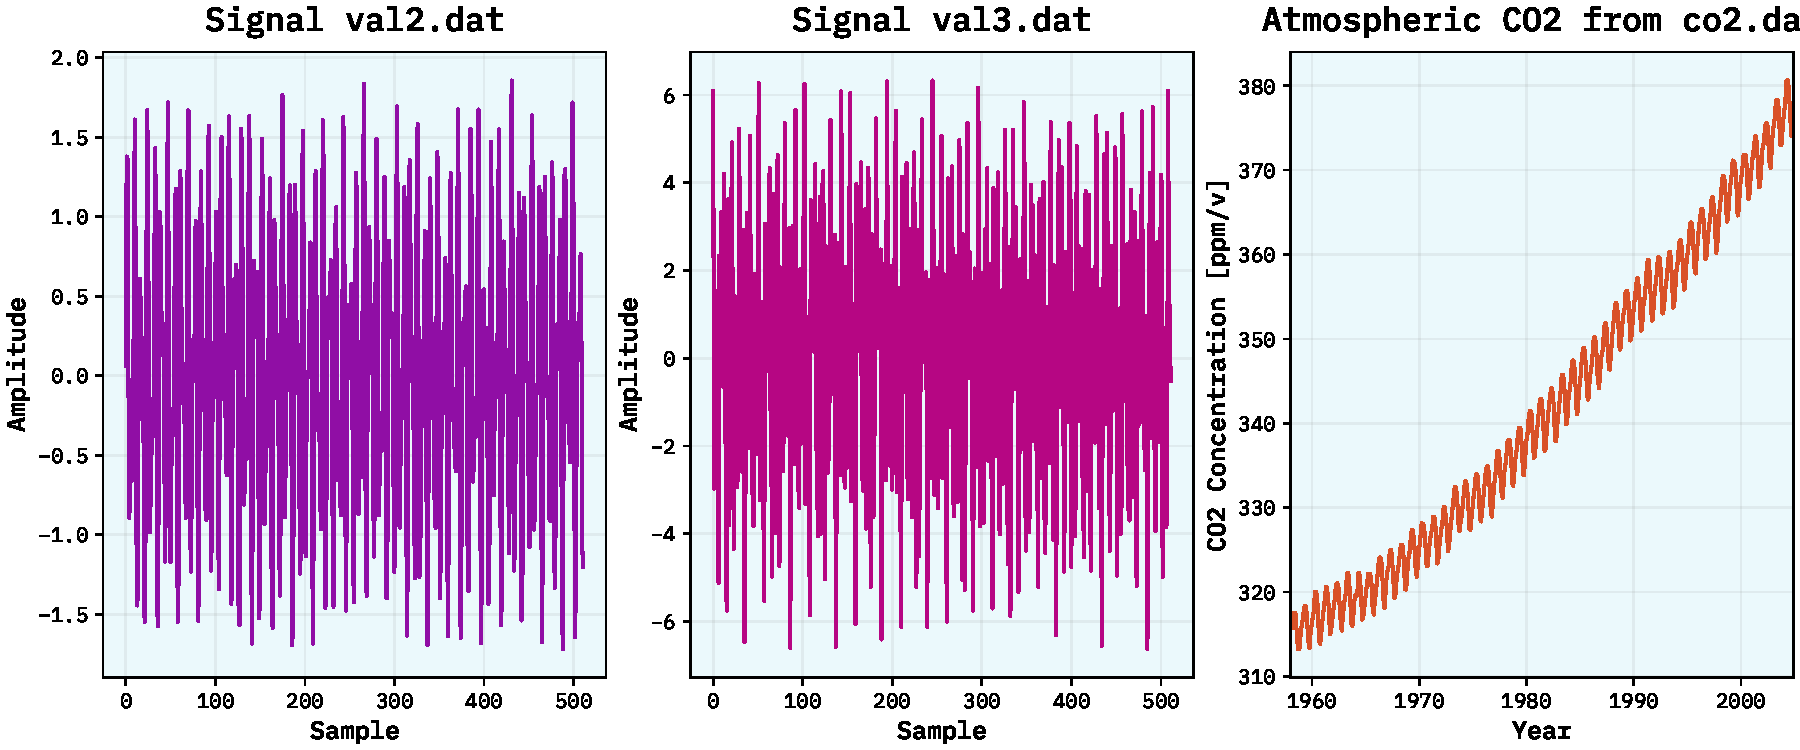
\includegraphics[width=0.95\textwidth]{../MaxEntropy/Images/supplied-data.pdf}
    \caption{The signals that we'll be analyzing in the first subtask.}
    \label{fig:signals}
\end{figure}

The instructions also want us to explore the various properties of the AR model and how it behaves when we change the
order of the model as well as the number of points we use to evaluate the spectra. The spectra can be calculated 
using the following formula:
%
\begin{equation}
    S(f) = \frac{1}{|1 - \sum_{i=1}^p a_i e^{-2\pi i f i}|^2}\>,
\end{equation}
%
however I used the \texttt{scipy.signal.freqz} for ease of use and to avoid any mistakes. 

\section{Solution Overview}
\section{Results}
\section{Conclusion and Comments}

% Add references
% \newpage
% \bibliographystyle{unsrt}
% \bibliography{mod112}

% End document
\end{document}
